\documentclass[a4]{article}
\usepackage{graphicx} 
\author{Group 7, System Black}
\title{Software Requirements Specification}

\begin{document}
\maketitle
\section{Introduction}


\section{Members}
(In Alphabetical Order)
\begin{itemize}
\item Qi, ZHU

\item Shijia, WEI

\item Shiyi, ZHU

\item Tao, LIN

\item Ye, QI
\end{itemize}


\section{Description}

\subsection{User Scenarios}
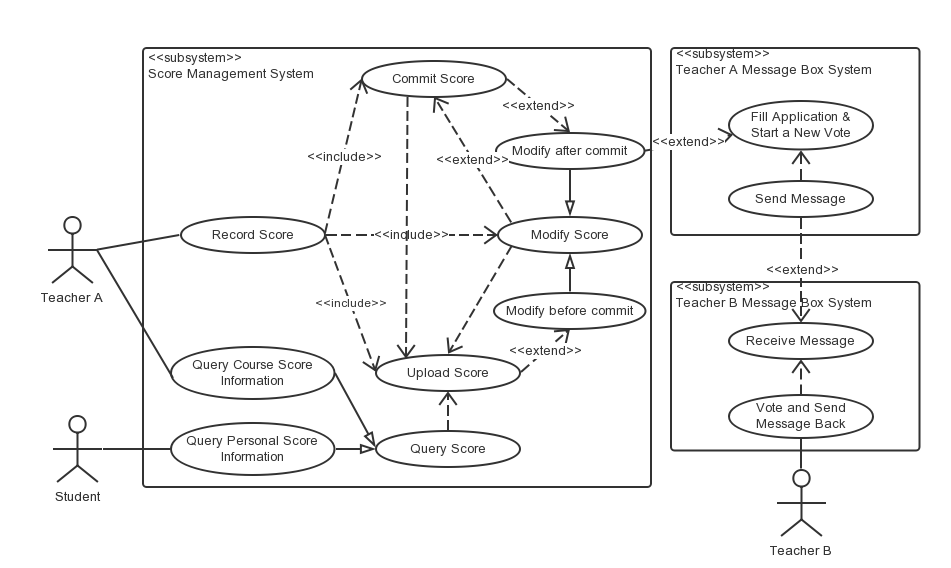
\includegraphics[width=5in]{pic/1.png}
\subsection{Data Flow Diagram}
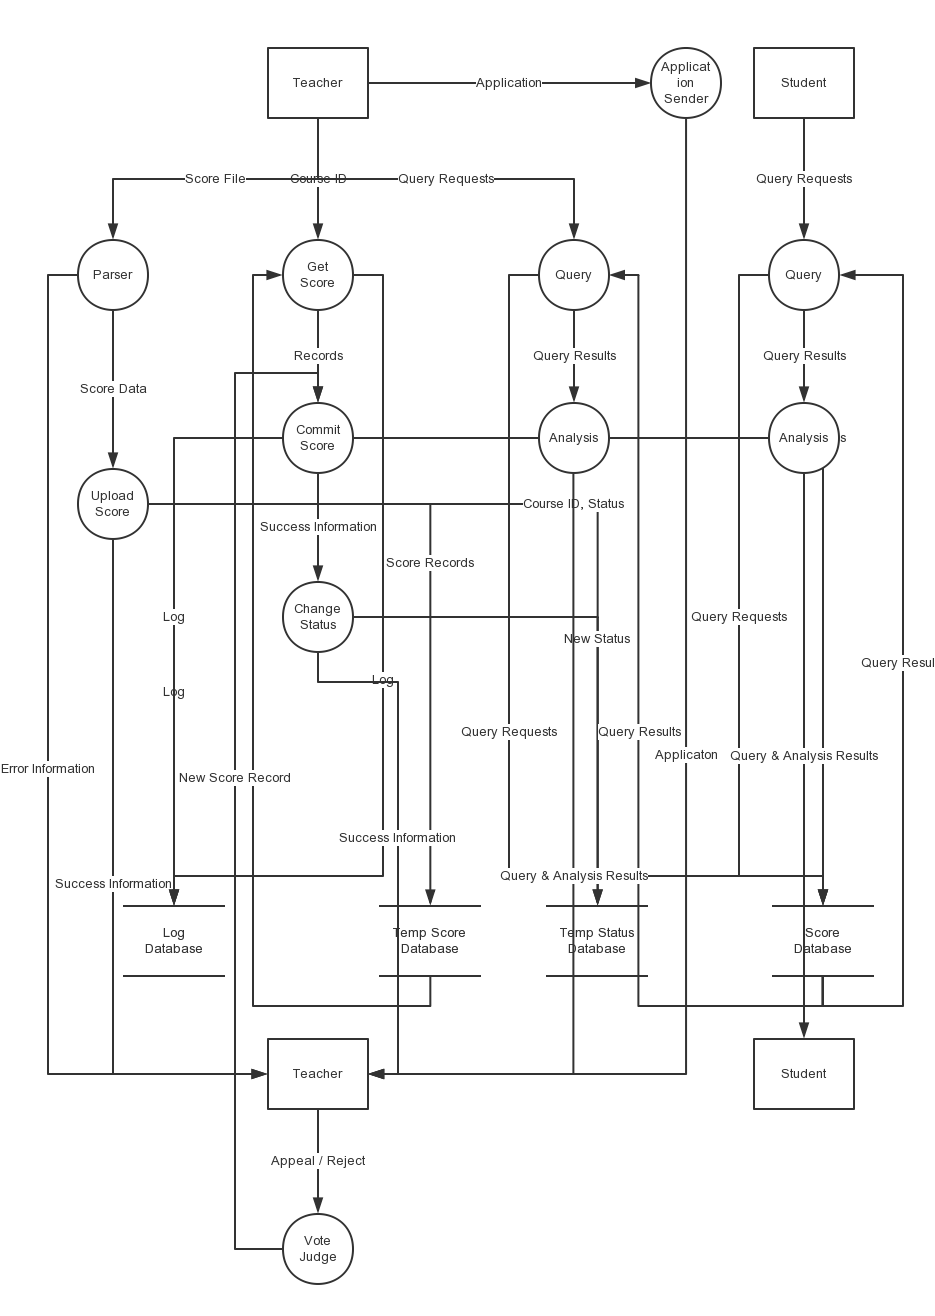
\includegraphics[width=5in]{pic/2.png}
\subsection{State Diagrams}
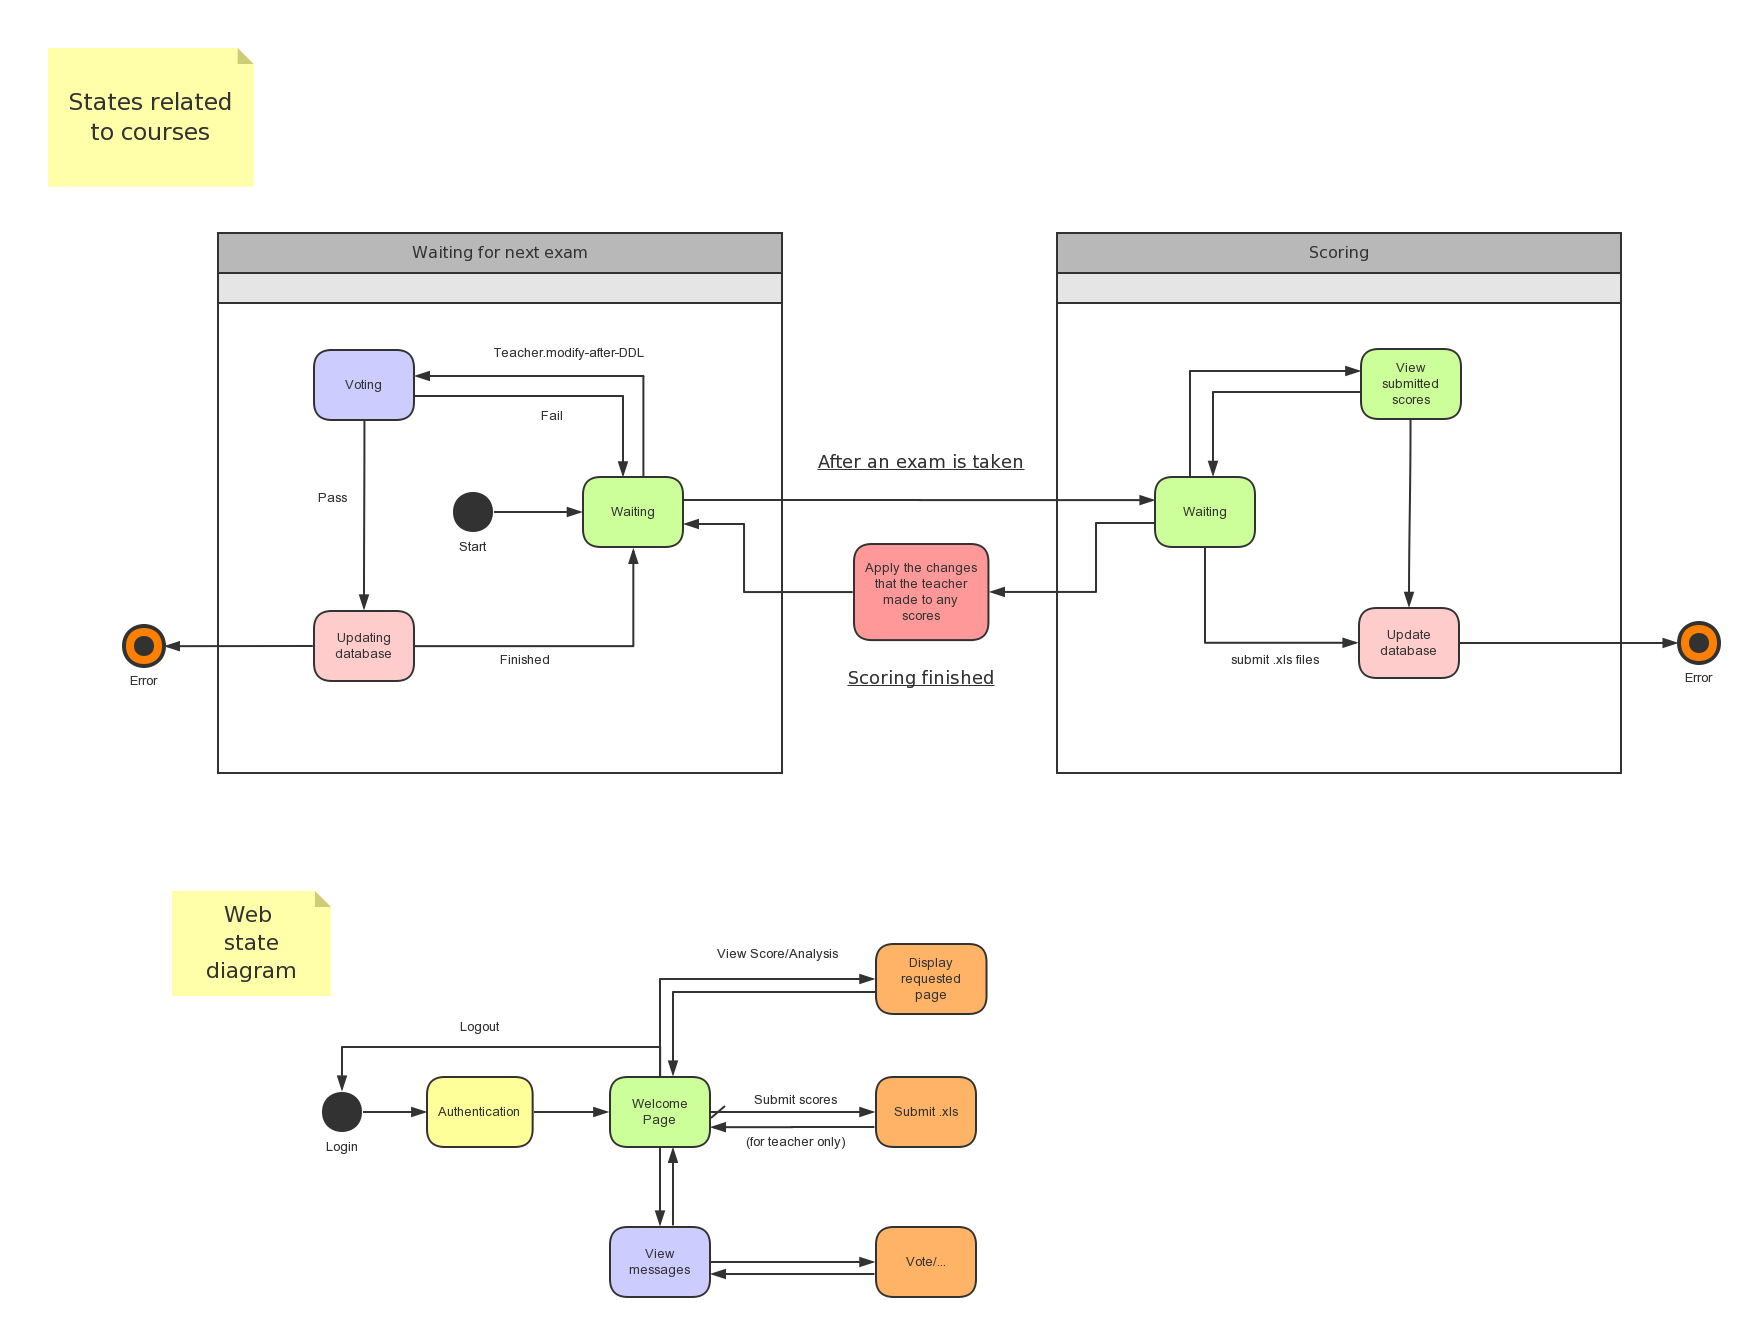
\includegraphics[width=5in]{pic/3.png}
\subsection{Class Diagrams}
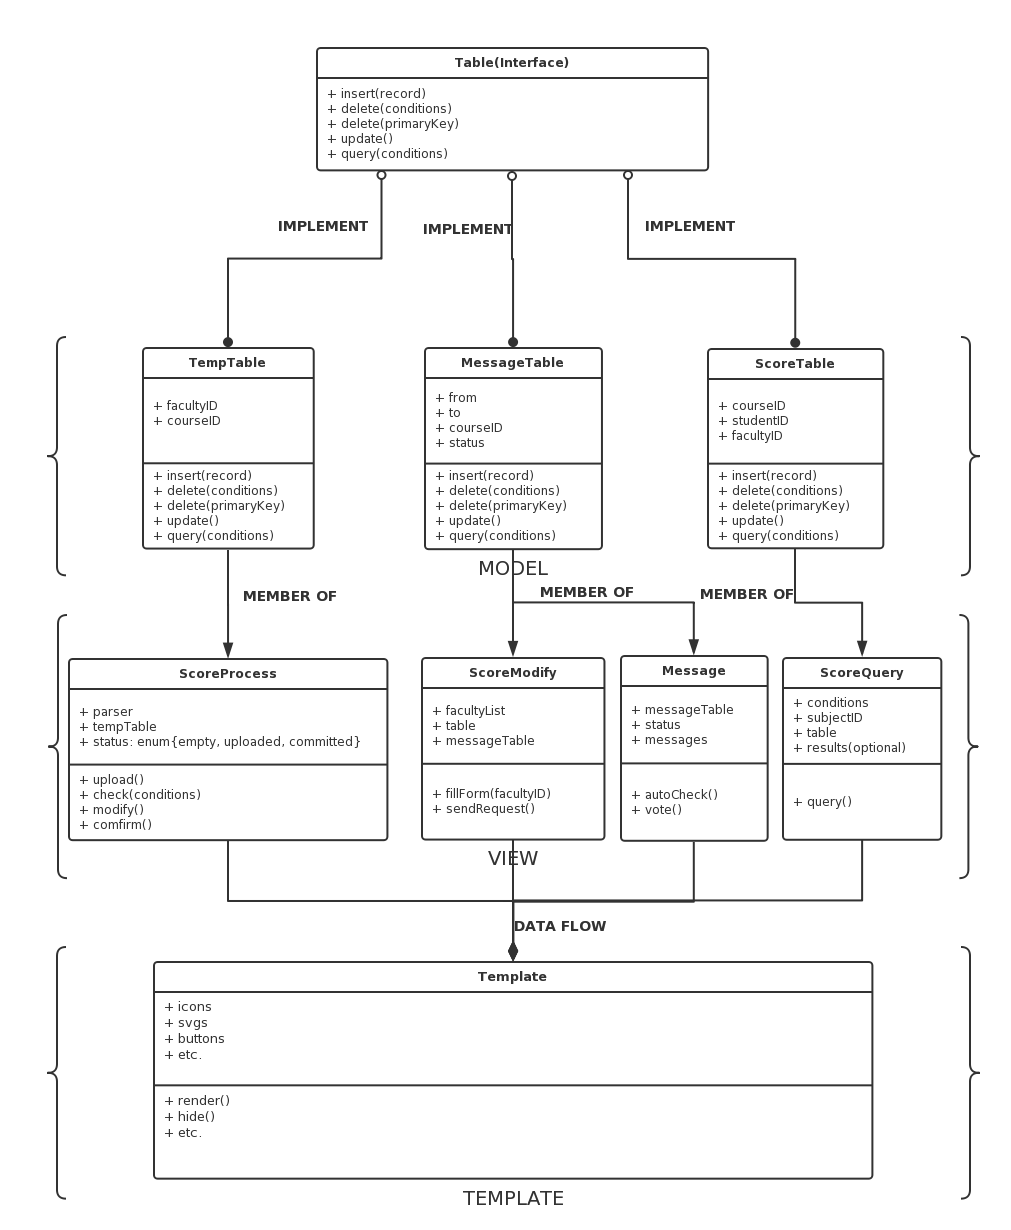
\includegraphics[width=5in]{pic/4.png}
\subsection{CRC Cards}
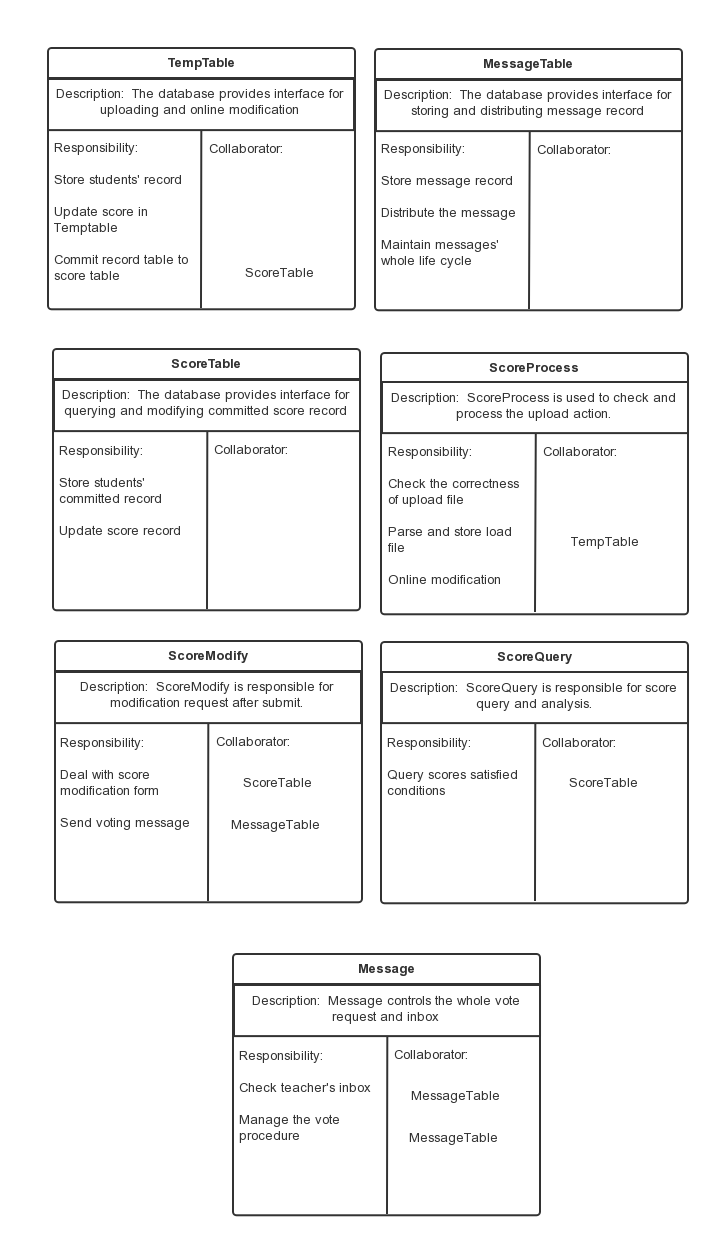
\includegraphics[width=5in]{pic/5.png}

\section{Validation Criteria}

\subsection{Defintion}
\begin{itemize}
\item \emph{Class:} A course instructed by a instructor in a semester.
\item \emph{Relevant Instructor:} The instructor who instructs the same course.
\end{itemize}

\subsection{Functions for Instructors}
\subsubsection{Record Scores}
\begin{enumerate}
\item An instructor could check the information of the classes he/she is currently instructing.
\item An instructor could download a transcript template to be filled from the system.
\item If the format of the transcript meets the criterion, it will be immediately parsed and shown on the screen in tabular form, with class status altered to ``UPLOADED''; otherwise, it will be rejected with detailed reason specified.
\item Any new uploading will directly cover previous files.
\item The scores of the class marked as ``UPLOADED'' could be browsed.
\item The scores of the class marked as ``UPLOADED'' could be directly modified online.
\item Having committed the scores of one class, an instructor could view the statistical information of it, with the class status altered to ``COMMITTED''.
\item The scores of the class marked as ``COMMITTED'' could only be browsed but not be directly modified.
\end{enumerate}

\subsubsection{Vote Modification}
\begin{enumerate}
\item If an instructor wants to modify the scores of a class marked as ``COMMITTED'', he/she needs to fill an online application form including course name, names of students whose scores need modification, new scores and corresponding reasons. All the relevant instructor will be apprised of this request.
\item The relevant instructors can vote for the request for score modification: they could choose either to approve it or to reject it.
\item If all of the relevant instructors agree with this modification, this request will be adopted and the instructor who starts it will get a notification telling the result.
\end{enumerate}
\subsubsection{Query/Analysis Scores}
This is valid after one specific class is marked as ``SUBMITTED''.
\begin{enumerate}
\item The instructor could view score distribution in graphic chart from.
\item The instructor could view ranking statistics in list chart from, including student names, raw scores and grade points.
\item The instructor could view average score in eye-catching place.
\end{enumerate}
\subsection{Functions for Students}
\subsubsection{Query/Analysis Scores}

\begin{enumerate}
\item A student could view score information of all classes that he/she has registered and is marked as ``SUBMITTED''. The score information includes course names, raw scores and grade points.
\item A student could view his/her GPA, average scores, total credits of the current semester.
\item A student could view his/her GPA, average scores, total credits of the courses he/she major in. 

\end{enumerate}


\end{document}


